\documentclass[letterpaper,12pt,fleqn]{article}
\usepackage{matharticle}
\pagestyle{plain}
\begin{document}

\begin{center}
\Large Math-08 Homework \#15 Solutions
\end{center}

\vspace{0.5in}

\underline{Reading}

\begin{itemize}
\item Text book section 5.1-5.3
\end{itemize}

\underline{Problems}

\begin{enumerate}

\item Consider the following system of equations:
  \[x^2+y^2-4x-6y-12=0\]
  \[x-y+6=0\]
  \begin{enumerate}
  \item Determine the points of intersection (if any).

    We use the substitution method. First, solve the second equation for $y$:
    \[y=x+6\]
    Now plug into the first equation and solve for $x$:
    \begin{eqnarray*}
      x^2+(x+6)^2-4x-6(x+6)-12 &=& 0 \\
      x^2+x^2+12x+36-4x-6x-36-12 &=& 0 \\
      2x^2+2x-12 &=& 0 \\
      x^2+x-6 &=& 0 \\
      (x+3)(x-2) &=& 0 \\
      x &=& -3,2
    \end{eqnarray*}
    Now plugging the found $x$ values into the second equation for solve for
    $y$:
    \[y=-3+6=3\]
    \[y=2+6=8\]
    So, the points of intersection are: $(-3,3)$ and $(2,8)$

  \item Give a geometric description of the problem - what are the
    geometric figures involved, what are the possibilities of intersection
    (there are three), and which of those possibilities is represented by the
    problem.

    This system represents a line intersecting a circle. There are three
    possible ways that this can happen:

    \begin{minipage}{2in}
      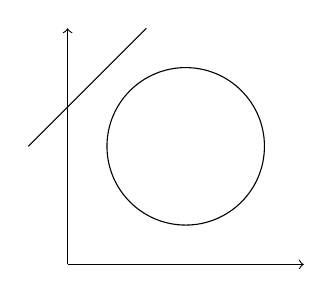
\begin{tikzpicture}
        \draw [->] (0,0) -- (3,0);
        \draw [->] (0,0) -- (0,3);
        \draw (1.5,1.5) circle [radius=1];
        \draw (-0.5,1.5) -- (1,3);
      \end{tikzpicture}

      No intersection
    \end{minipage}
    \begin{minipage}{2in}
      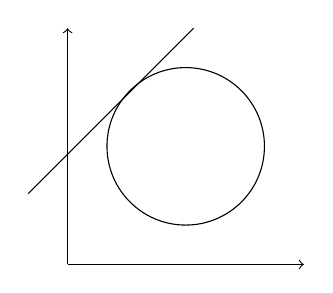
\begin{tikzpicture}
        \draw [->] (0,0) -- (3,0);
        \draw [->] (0,0) -- (0,3);
        \draw (1.5,1.5) circle [radius=1];
        \draw (-0.5,0.9) -- (1.6,3);
      \end{tikzpicture}

      1 point
    \end{minipage}
    \begin{minipage}{2in}
      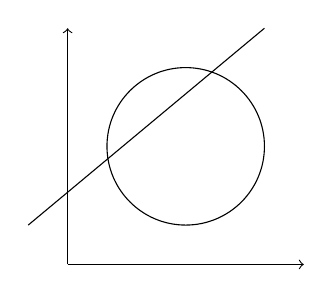
\begin{tikzpicture}
        \draw [->] (0,0) -- (3,0);
        \draw [->] (0,0) -- (0,3);
        \draw (1.5,1.5) circle [radius=1];
        \draw (-0.5,0.5) -- (2.5,3);
      \end{tikzpicture}

      2 points
    \end{minipage}

    Note that since the circle is not linear, we are not bound by the
    $0,1,\infty$ solutions rule. Our particular case is the third one -
    intersection at two points.
  \end{enumerate}

\item Solve the following system of linear equations:
  \[3x+3y+5z=1\]
  \[3x+5y+9z=0\]
  \[5x+9y+17z=0\]
  You may use row operations directly on the equations, or use a matrix. For
  each step, clearly indicate the row operation used and state of the
  equations/matrix after the row operation.

  \[\left[\begin{array}{ccc|c}
      3 & 3 & 5 & 1 \\
      3 & 5 & 9 & 0 \\
      5 & 9 & 17 & 0
    \end{array}\right]\]

  $-R_1+R_2\to R_2$
  \[\left[\begin{array}{ccc|c}
      3 & 3 & 5 & 1 \\
      0 & 2 & 4 & -1 \\
      5 & 9 & 17 & 0
    \end{array}\right]\]

  $\frac{1}{3}R_1\to R_1$ \\
  $\frac{1}{2}R_2\to R_2$
  \[\left[\begin{array}{ccc|c}
      1 & 1 & \frac{5}{3} & \frac{1}{3} \\
      0 & 1 & 2 & -\frac{1}{2} \\
      5 & 9 & 17 & 0
    \end{array}\right]\]

  $-5R_1+R_3\to R_3$
  \[\left[\begin{array}{ccc|c}
      1 & 1 & \frac{5}{3} & \frac{1}{3} \\
      0 & 1 & 2 & -\frac{1}{2} \\
      0 & 4 & \frac{26}{3} & -\frac{5}{3}
    \end{array}\right]\]

  $-4R_2+R_3\to R_3$
  \[\left[\begin{array}{ccc|c}
      1 & 1 & \frac{5}{3} & \frac{1}{3} \\
      0 & 1 & 2 & -\frac{1}{2} \\
      0 & 0 & \frac{2}{3} & \frac{1}{3}
    \end{array}\right]\]

  $\frac{3}{2}R_3\to R_3$
  \[\left[\begin{array}{ccc|c}
      1 & 1 & \frac{5}{3} & \frac{1}{3} \\
      0 & 1 & 2 & -\frac{1}{2} \\
      0 & 0 & 1 & \frac{1}{2}
    \end{array}\right]\]

  We can now back-solve:
  \begin{eqnarray*}
    x+y+\frac{5}{3}z &=& \frac{1}{3} \\
    y+2z &=& -\frac{1}{2} \\
    z &=& \frac{1}{2}
  \end{eqnarray*}
  \begin{eqnarray*}
    z &=& \frac{1}{2}
  \end{eqnarray*}
  \begin{eqnarray*}
    y+2(\frac{1}{2}) &=& -\frac{1}{2} \\
    y+1 &=& -\frac{1}{2} \\
    y &=& -\frac{3}{2} \\
  \end{eqnarray*}
  \begin{eqnarray*}
    x+(-\frac{3}{2})+\frac{5}{3}(\frac{1}{2}) &=& \frac{1}{3} \\
    x-\frac{3}{2}+\frac{5}{6} &=& \frac{1}{3} \\
    x-\frac{2}{3} &=& \frac{1}{3} \\
    x &=& 1
  \end{eqnarray*}

  Solution: $\left(1,-\frac{3}{2},\frac{1}{2}\right)$
\end{enumerate}
\end{document}
